% \begin{figure}
%     \centering
%         \begin{subfigure}[b]{0.49\textwidth}
%          \centering
%          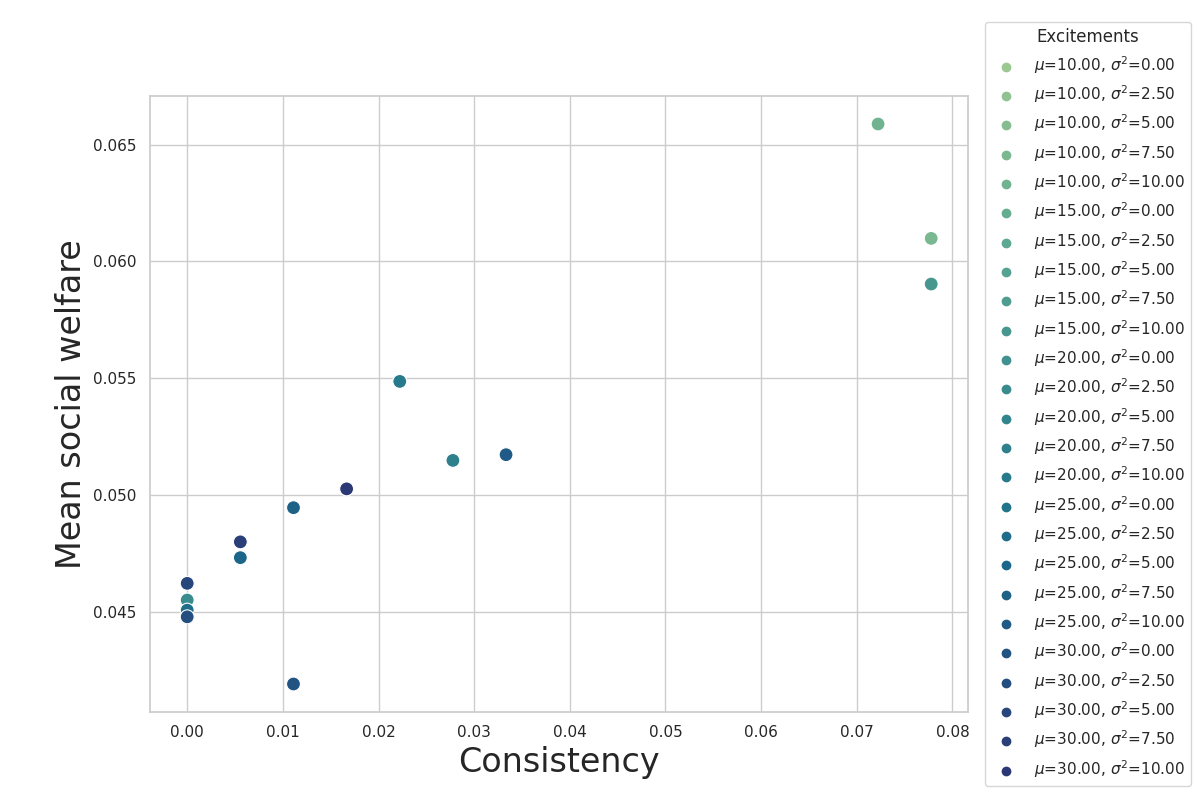
\includegraphics[width=\textwidth]{figures/mpda_dynamics_initliazation.png}
%          \caption{Dynamic Initialization}
%          \label{fig:init}
%         \end{subfigure}
%          \begin{subfigure}[b]{0.49\textwidth}
%          \centering
%          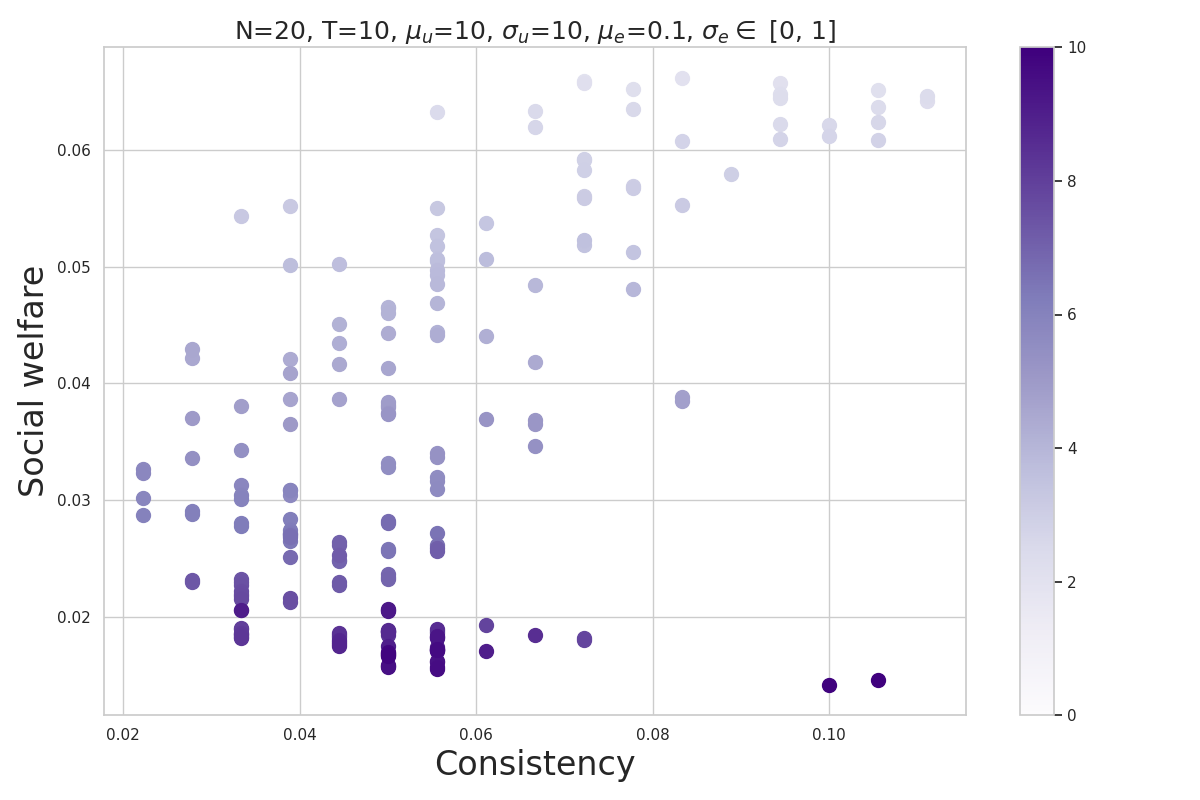
\includegraphics[width=\textwidth]{figures/mpda_dynamics_excitement_std.png}
%          \caption{Dynamic Excitement}
%          \label{fig:excite_std}
%      \end{subfigure}
%          \begin{subfigure}[b]{0.49\textwidth}
%          \centering
%          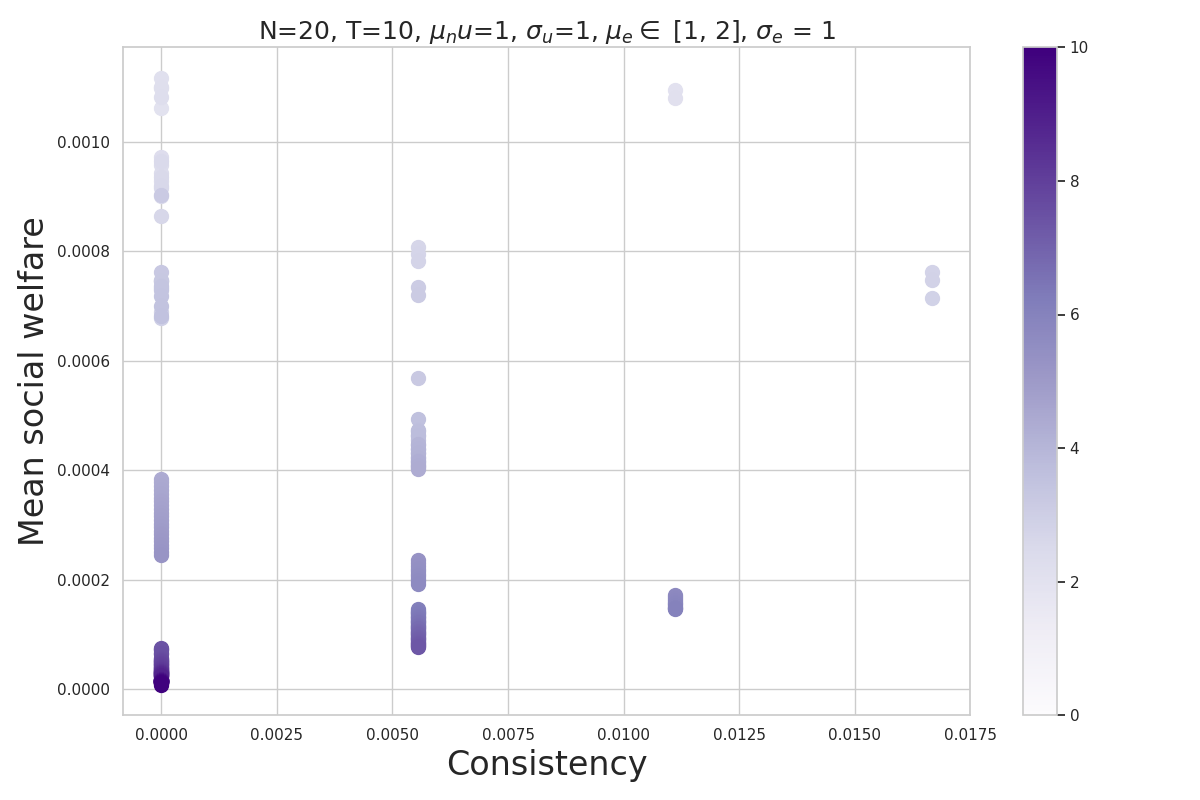
\includegraphics[width=\textwidth]{figures/mpda_dynamics_excitement_mean.png}
%          \caption{Dynamic Excitement}
%          \label{fig:excite_mean}
%      \end{subfigure}
%      \caption{Mean social welfare vs. consistency for MPDA applied to two dyanmic scenarios; (a) fixed excitement; (b) fixed initialization varying excitement (fixed mean); (c) fized initialization with varying excitement (fixed standard deviation).}
%     \label{fig:mpda_dynamics}
% \end{figure}
\begin{figure}
    \centering
    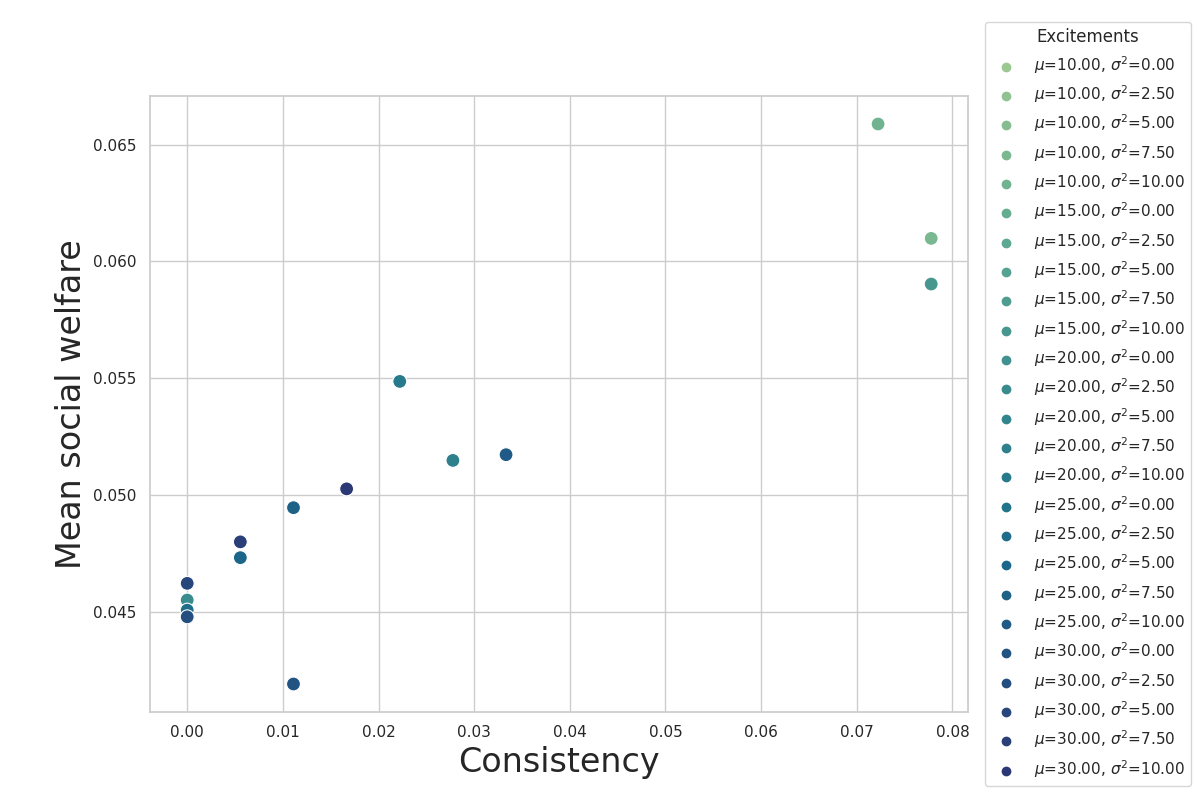
\includegraphics[width=0.32\linewidth]{figures/mpda_dynamics_initliazation.png}
    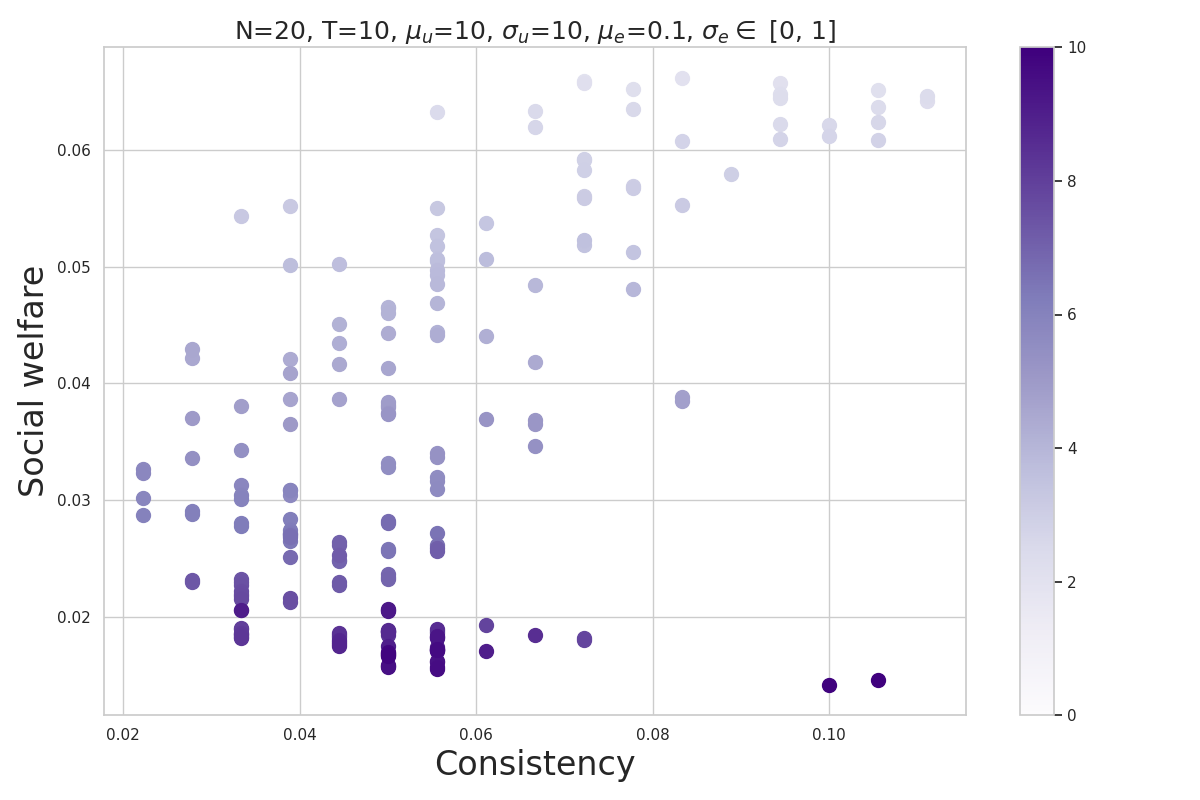
\includegraphics[width=0.32\linewidth]{figures/mpda_dynamics_excitement_std.png}
    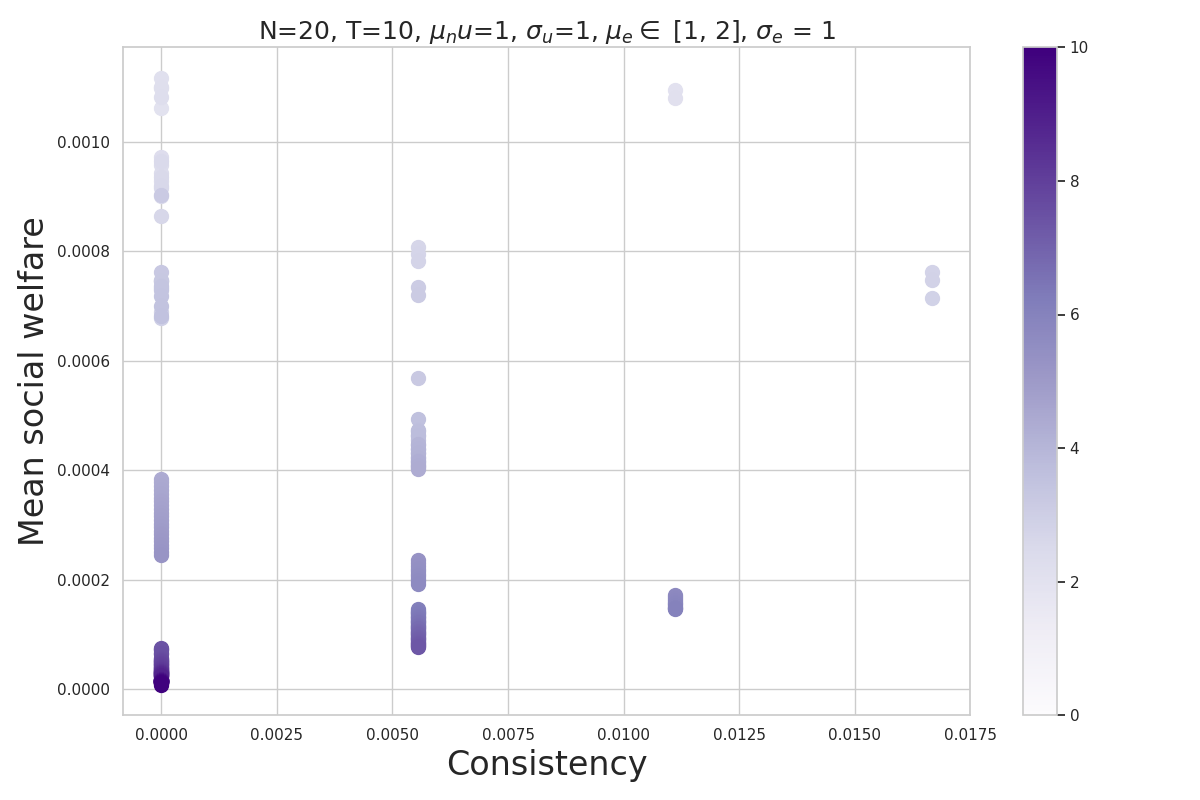
\includegraphics[width=0.32\linewidth]{figures/mpda_dynamics_excitement_mean.png}
     \caption{Mean social welfare vs. consistency for MPDA applied in various settings with 20 men/women and 10 time steps. (Left) Fixed excitement with varying utilities initialization (fixed mean). (Middle) Fixed utilities initialization but varying excitement (fixed mean) (b) fixed initialization varying excitement (fixed mean). (Right) Fixed utilities initialization but varying excitement (fixed variance).}
    \label{fig:mpda_dynamics}
\end{figure}